\chapter{Proposed Analysis Approaches}
\label{CHAP:methods}

A variety of methods have been proposed in the literature to analyse survival endpoints in clinical trials when treatment switching occurs. This chapter reviews the main methods proposed based primarily on those discussed within \cite{TSD16}. First considering those described as simple and then those described as complex. In this chapter I describe the analysis approaches, their key assumptions and some unclear aspects of implementation that will be investigated through simulation.

\section{Simple approaches}

\subsection{Intention-To-Treat (ITT) analysis}
Commonly in papers describing treatment switching reference is made to the ITT analysis. In the context of treatment switching this refers to analysing the trial results as observed and essentially ignoring that switching took place. If the experimental treatment is effective then this analysis could underestimate the true treatment effect. The magnitude of this bias will depend on the extent of the treatment switching both in terms of duration of exposure to switch treatment and proportion of patients exposed. 

\subsection{Per-protocol analysis}
Two similar approaches can be considered as per-protocol analysis as they exclude or censor data from patients who switch from the analysis. They both have the advantage that they are simple to implement in standard statistical software.

\subsubsection{Censoring at Crossover}
In this approach patients are censored at the time they switch treatment. The key assumption made is that this censoring is non-informative meaning that the outcome being analysed is independent of the switching. \cite{TSD16} challenge this assumption stating that ``clinicians decide whether it is appropriate for individual patients to switch and this decision will be made based upon patient characteristics rather than being random''. 

\subsubsection{Excluding Switchers}
For this analysis patients who switch are excluded from the analysis. This breaks the randomization and as \cite{Watkins2013} note ``makes the assumption that the control arm switchers and non-switchers have the same prognosis'' which as noted previously is an assumption that \cite{TSD16} challenge. \cite{Watkins2013} also highlight that ``Patients also have to live long enough to be able to switch, so longer-living individuals are removed.'' further creating the potential for bias to be introduced into the analysis.

\subsection{Time-dependent Cox proportional hazards model}

A further approach is to include treatment exposure as a time varying covariate into a Time dependent Cox-model. Such models can be easily fit with standard statistical software. However, while easy to implement \cite{Watkins2013} note this approach will be biased ``If there are confounding variables that influence both the time-varying treatment covariate and survival.'' While in a non-oncology setting \cite{Hernan2000} are explicit that:
\begin{quote}
[the time-dependent Cox proportional hazards model] approach may be biased, whether or not one further adjusts for past covariate history, whenever (1) there exists a time-dependent covariate that is both a risk factor for mortality and also predicts subsequent exposure and (2) past exposure history predicts the risk factor.
\end{quote}
In the context of oncology clinical trials \cite{TSD16} state that it is highly likely that ``switching is associated with prognostic patient characteristics''. It is clear that such prognostic patient characteristics would be confounding variables by this definition and therefore the time varying covariate analysis may be biased even if adjusted for these characteristics.

A potential variation of this approach that may address these limitations is where two covariates are considered for treatment: one for randomized treatment that is not time dependent and a second covariate for exposure to experimental therapy as a switch therapy that is time dependent as described by \cite{Leon2014}. 

\section{Inverse Probability of censoring Weights (IPCW)}

The analysis method or IPCW described by \cite{Robins2000} censors information that occurs after treatment switch. In order to avoid the selection bias that can confound the per-protocol analysis of censoring at treatment switch observations that are not censored are weighted to create a pseudopopulation with the same characteristics as the overall trial population. To do this a model is built to predict censoring based on observed covariates over time which is used to estimate for each patient the conditional probability of remaining uncensored. The inverse of this estimated probability is then used as a weight into the estimation of a corrected hazard ratio. 

\subsection{Model for censoring}

The model for censoring can be in either discrete or continuous time. The primary benefit of using discrete time is the ease of calculation in standard software such as the demonstrations by \cite{Hernan2000} or \cite{Fewell2004}. In the case of discrete time the model for probability of censoring is of the form shown in Equation \ref{E:chap_methrev:IPCWcm}. Where $\mathbb{P}(C=1|t)$ indicates the probability of being censored in interval $t$, with $t=0,1, \ldots, T$ representing discrete time intervals, $X_t$ is a vector of time dependent covariates and $X_0$ is a vector of baseline covariates and the $\beta$ terms can be estimated through e.g. pooled logistic regression including each patient multiple times.

\begin{equation}
\label{E:chap_methrev:IPCWcm}
\mathbb{P}(C=1|t) = \alpha_t + \beta_0^\prime  X_0 + \beta^\prime X_t 
\end{equation}

It can be seen that this model requires covariates ($X_t$) for each patient for all time periods until censoring (or death). While for patients who switch this may be feasible for patients who do not switch it is unclear if this feasible. In practice it may be necessary to replace the covariate values by predicted values from a mixed effect repeated measures model of the covariate over time (making additional assumptions about any missingness).

\subsection{Estimating the weights}

By multiplying the probability of being uncensored in each time period the cumulative probability of being uncensored at each time for each patient can be estimated. For unstabilized weights the inverse of this probability is taken while for stabilized weights the same process is used but instead of the numerator being 1 the numerator is based on the probability of being uncensored given only baseline covariates. As such the formula for unstabilized weights is shown in Equation \ref{E:chap_methrev:IPCW.W} and for stabilized weights in Equation \ref{E:chap_methrev:IPCW.SW}. 

\begin{equation}
\label{E:chap_methrev:IPCW.W}
\hat{W}(t) = \prod^t_{k=0} \frac{1}{1-\mathbb{P}(C=1|k, X_0, X_k)}
\end{equation}

\begin{equation}
\label{E:chap_methrev:IPCW.SW}
\hat{W}(t) = \prod^t_{k=0} \frac{1-\mathbb{P}(C=1|k, X_0)}{1-\mathbb{P}(C=1|k, X_0, X_k)}
\end{equation}

\subsection{Model requirements}

\cite{Cole2008} identifies the key requirements for this model to yield valid estimates as Exchangeability and Positivity. Exchangability simply means that all covariates that influence censoring and outcome are captured in the weight estimation model and that given these covariates over time any given patient is exchangeable with another having the same covariate history. This is commonly referred to as the no unmeasured confounders assumption by \cite{TSD16} and others. The second requirement of Positivity is defined by \cite{Cole2008} as ``the condition that there are both exposed and unexposed individuals at every level of the confounders.''. It can be seen that these two conditions can be in conflict particularly in the presence of small sample sizes (such as a clinical trial) whereby each additional covariate introduced to improve the exchangeability assumption will increase the possibility of creating a level of covariates for which the probability of being censored is 0 or 1 violating the positivity assumption. This issue has been shown in practice in the simulation study of \cite{Latimer2013} where scenarios with very high switching proportions lad to large bias as no patients existed to replace those who switched.

\subsection{Estimating a corrected Hazard Ratio}

After weights by patient and time have been estimated it is possible to include them into a time dependent weighted Cox model driectly or into a weighted generalized linear model using a complementary log-log link to estimate a hazard ratio as shown by \cite{Hernan2000}. In this model patients who switch treatment are censored at the time of switch.

\section{Rank Preserving Structural Failure Time (RPSFT) models}

\cite{Robins1991} introduced a randomization based approach to address treatment non-compliance in clinical trials. It considers 3 different survival times for a patient $i$:
\begin{enumerate}
\item $T_i$ which is their observed survival time given their observed treatment history
\item $U_i$ which is their ``latent'' survival time  under no treatment. This is an unobserved baseline variable.
\item $V_i$ which is their ``counter-factual'' survival time under some different treatment history than that observed. 
\end{enumerate}
An RPSFT model is then defined to relate these survival times and enable the estimation of $V_i$. 

\subsection{The RPSFT model}
The general form of the RPSFT model is shown in Equation \ref{E:rpsft1}. Here I deviate from the notation used by \cite{Robins1991} where they define a model $\psi()$ with parameters $\beta$ wheras I follow here the convention commonly in later papers e.g. \cite{White1999}, \cite{Morden2011} or \cite{Watkins2013} to use $\psi$ to refer to the parameters of the model.  
\begin{equation}
\label{E:rpsft1}
U_i = f\left(T_i, H_i(T_i), \psi \right)
\end{equation}
$H_i()$ is a time dependent treatment history which for $H_i(T_i)$ is observed and $\psi \in \mathrm{R}^v, v \geq 1$ are unknown parameters. $f()$, the RPSFT model, is then a smooth function which satisfies the following criteria:
\begin{enumerate}
\item It is rank preserving so that $u_a = f(t_a,H_i(t_a),\psi) > u_b = f(t_b,H_i(t_b),\psi)$ if $t_a>t_b$ which means that if a patient $a$ with longer survival than $b$ with the same treatment history would also have longer survival when both had any other treatment history.
\item $t=f(t,H_i(t),\psi)$ if $H_i(t)$ is identically 0 on $(0,t)$ so without treatment the latent survival time is observed.
\item $t=f(t,H_i(t),0)$ so $\psi$ identically 0 implies no treatment effect.
\end{enumerate}
Given such a model $f$ where the parameters $\psi$ are known it is possible to estimate the latent survival times $U_i$ form the observed survival time $T_i$ and observed treatment history $H_i(T_i)$. These latent survival times can then be used to estimate $V_i^{(h)}$ the counter-factual survival times under another treatment history $(h)$. In the context of treatment switching this counter-factual treatment history would normally be where patients took only their randomized treatment. Equation \ref{E:rpsft2} shows this relationship. It is important to note that $V_i^{(h)}$ depends only on $U_i$ and not $T_i$ which will be considered further when discussing issues with censored data.
\begin{equation}
\label{E:rpsft2}
U_i = f\left(V_i^{(h)}, H^{(h)}_i(V_i^{(h)}),\psi\right)
\end{equation}

\subsubsection{Model assumptions}
Two key assumptions are made with this method. The first assumption is that the distribution of $U_i$ the latent survival time will be balanced by randomization between the randomized groups of the trial as it is a baseline characteristic. \cite{TSD16} notes that this assumption ``should be reasonable in the context of an RCT'' and that while important differences could occur in trials this maybe addressed through adjusting for prognostic covariates. The second assumption is that the RPSFT model chosen is correct. The specific form of the model chosen will therefore create its own assumptions.



\subsection{Model fitting}
Once the structural model relating $U$ and $T$ has been defined it is necessary to estimate the unknown parameters $\psi$. This is estimated through a process known as g-estimation. \cite{Robins1991} rely on the assumption that latent survival is balanced through randomization and use rank tests of the hypothesis that the $U_i$ are independent of randomized arm to define $\psi_0$ as the value where this hypothesis is true. \cite{KorhonenATBC}, \cite{White1999} and others describe the processes to get an estimate $\hat{\psi}$ of $\psi_0$ as follows.

\begin{enumerate}
\item Define a grid of candidate values for $\psi$.
\item For each $\psi$ estimate the latent survival time $U(\psi)$.
\item Compare the latent survival times as randomized with a suitable test (commonly a log-rank test) to get a test-statistic, $Z(U,\psi) = Z(\psi)$, for the difference in distributions of the $U$ comparing the control and experimental arms.
\item Choose $\hat{\psi}$ such that $Z(\hat{\psi}) \simeq Z(\psi_0)$, that is choose $\hat{\psi}$ such that the distribution of $U$ in the control arm is close to that of the distribution of $U$ in the experimental arm, ``the point estimate $\hat{\psi}$ is taken as the value closest to the null value where the test statistic reaches its minimum (or equivalently the p-value is at its maximum)'' \citep{KorhonenRECORD}. 
\end{enumerate}

This is illustrated in Figure \ref{F:C2:demo_g_est} for a simulated data set.
\begin{figure}[ht]
\centering
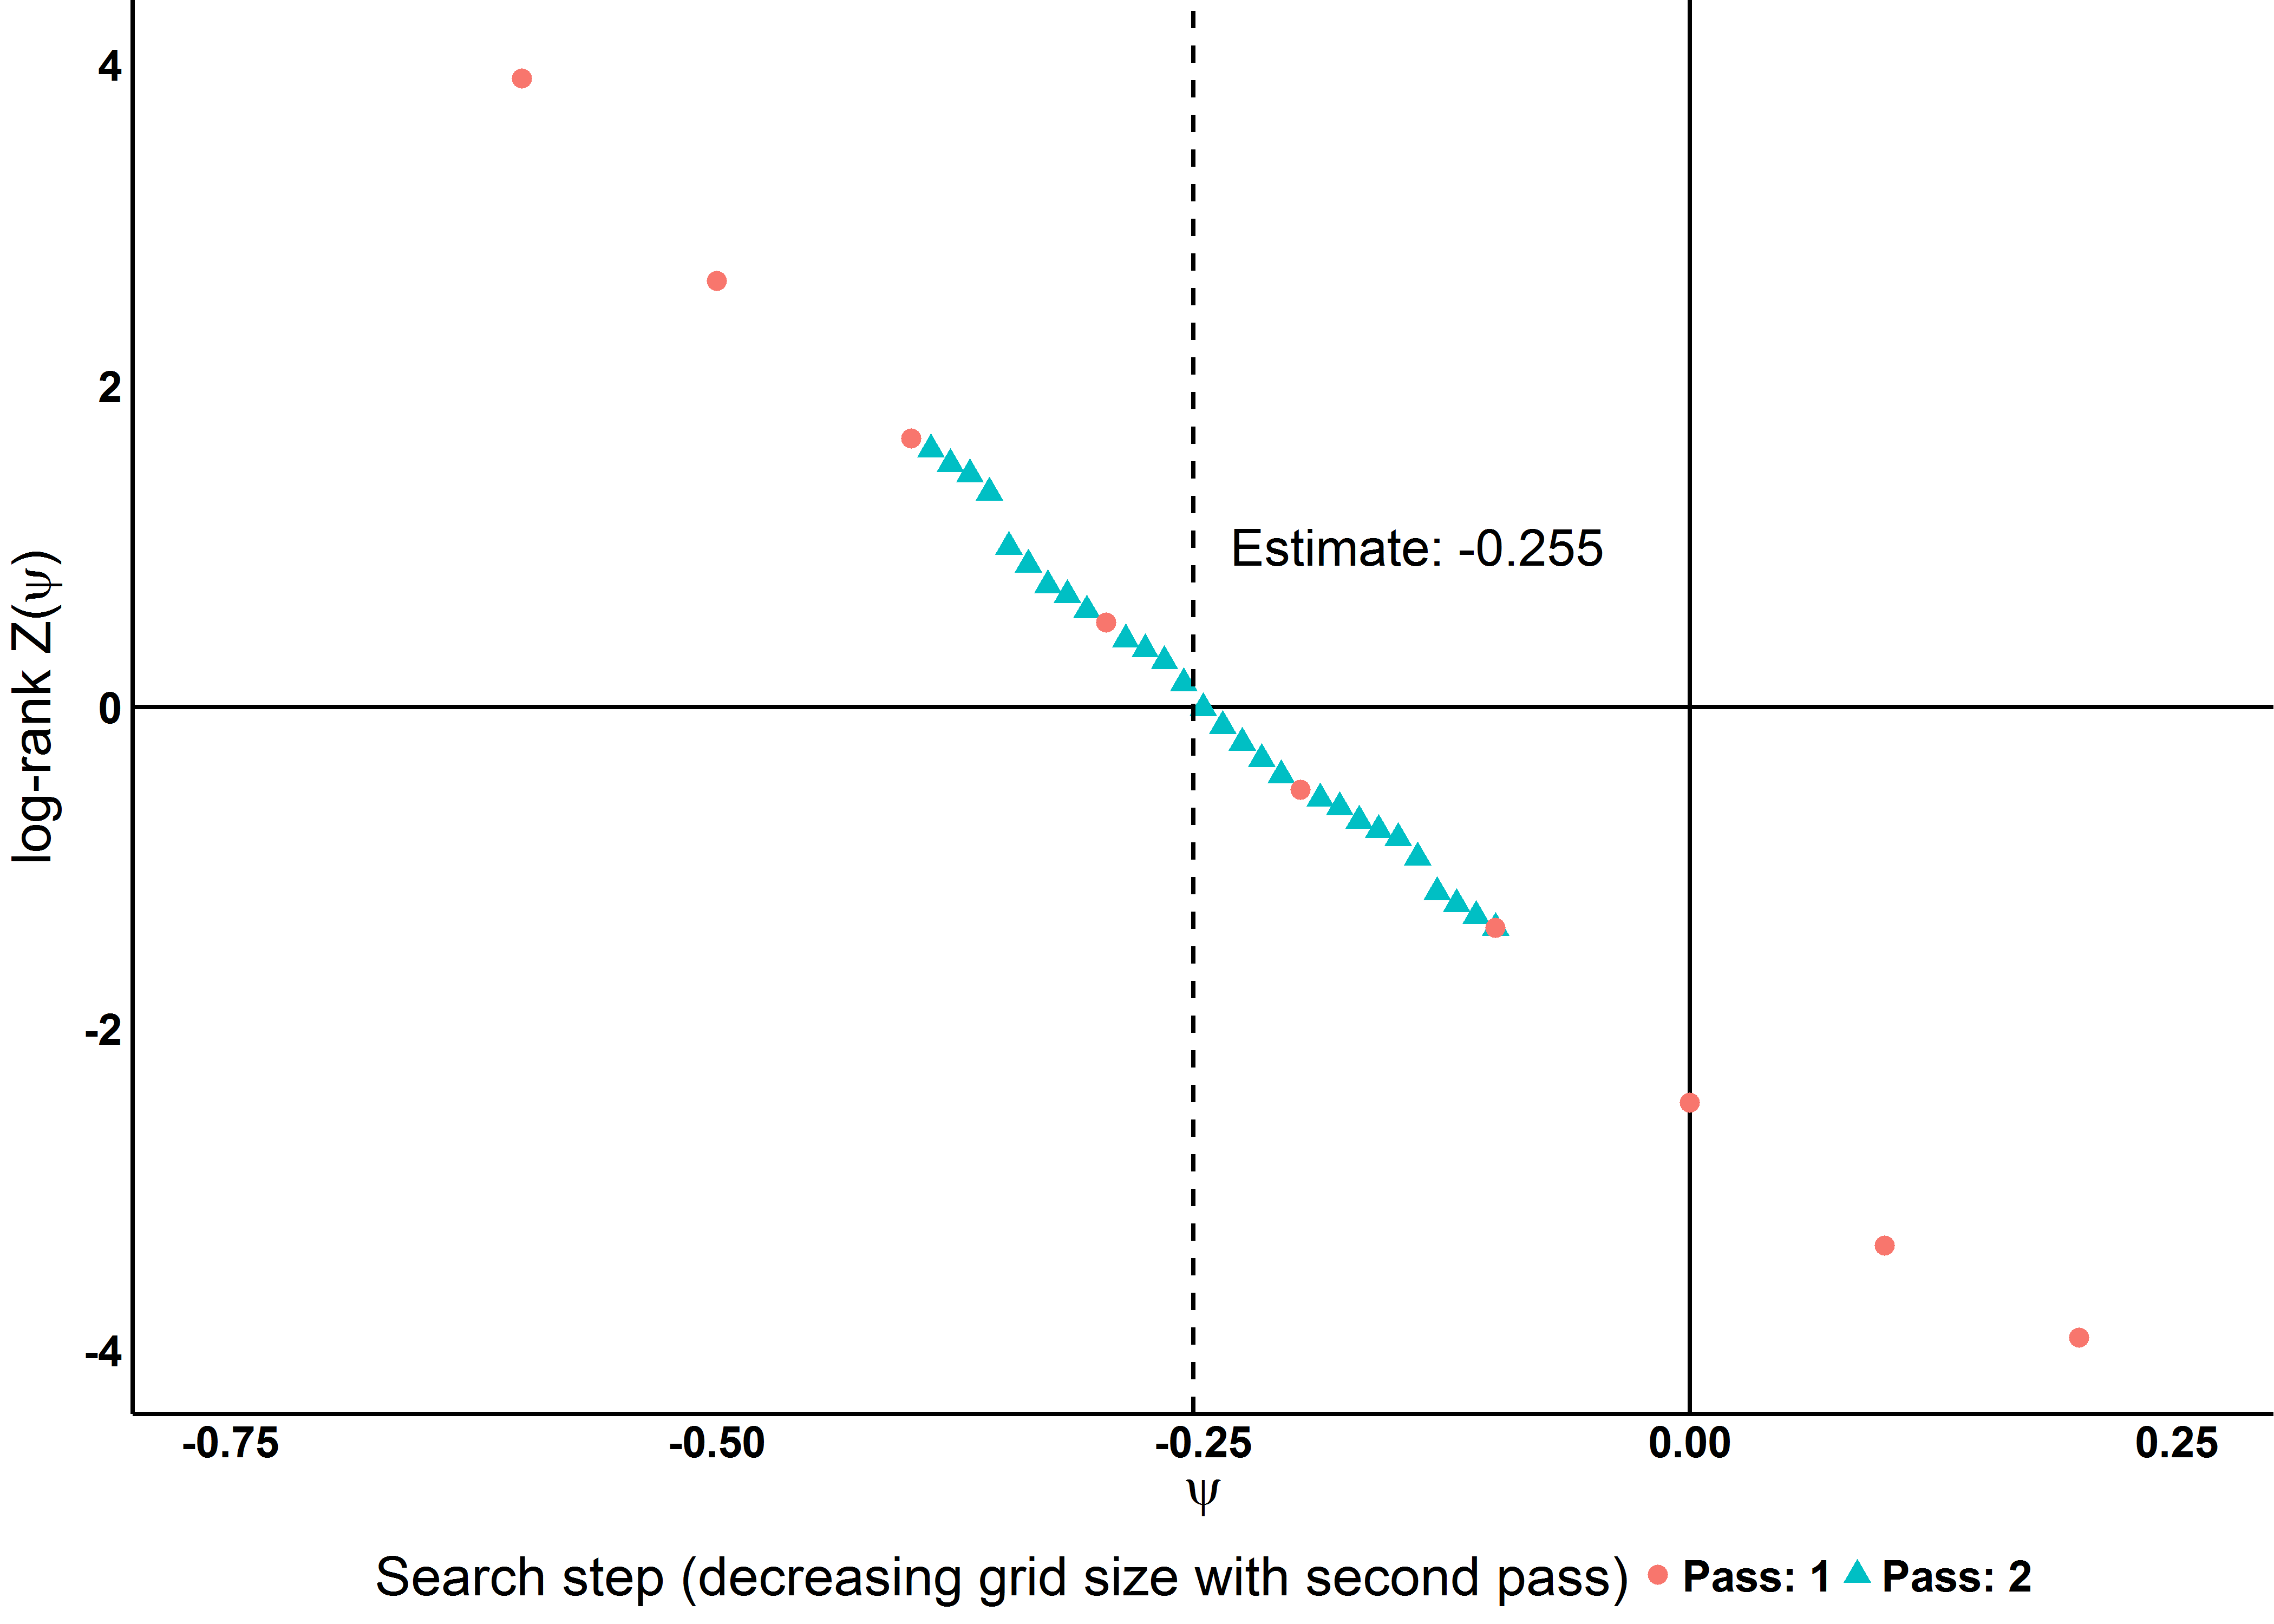
\includegraphics[width=13cm]{images/chap_methrev/example_g_est.png}
\caption{\label{F:C2:demo_g_est} Illustration of g-estimation using log-rank test statistic with $\hat{\psi}$ estimated as -0.255.} 
\end{figure}

\label{S:chap_methrev:RPSFTfit}

\subsubsection{Choice of test}

\cite{Robins1991} note for all datasets a locally most powerful test with a unique solution will exist, however, identifying this test is not trivial. \cite{TSD16} states that ``a log-rank or Wilcoxon test can be used for the RPSFTM g-test in a non-parametric setting [\ldots] or a Wald test could be used for parametric models''. In a non-parametric setting \cite{KorhonenRECORD} investigated the Fleming-Harrington family of rank tests which have a parameter $\rho$ and includes both log-rank ($\rho=0$) and Wilcoxon ($\rho=1$) tests and found that for their application ``[$\hat{\psi}$] is quite robust to different values of $\rho$''. 

\subsubsection{Issues with estimation}

\label{S:chap_methrev:ESTissues}
\cite{White1999} and \cite{White2002} identified a challenge in the g-estimation of $\hat{\psi}$ that as a rank test is used there may not be a solution where $Z(\psi)=0$.  Their proposed solution is to interpolate between the points where the sign of $Z(\psi)$ changes. It should be noted this is only possible when considering a test statistic that indicates a direction for the difference in survival times comparing the $U_i$ as randomized. As an example considering the log-rank test this means it is preferable to perform the g-estimation using the log-rank test statistic directly rather than use the $\chi^2$ value or $p$-value from the test. in addition they recommend an approach to take if multiple such crossing points are found:
\begin{quote}
We obtained a single point estimate $\hat{\psi}$ as follows. If the crossing points are $a_0$, $a_1$, $a_2$, \ldots, $a_n$ (where $n$ is even), then we took $\hat{\psi} = a_0 -a_1+a_2-\ldots+a_n$. This can be viewed as an average of the extreme crossing points $a_0$ and $a_n$, weighted by the length of time for which $Z(\psi)$ is positive and negative for $\psi$ in [$a_0$, $a_n$]
\end{quote}


\subsubsection{Handling Censored Data}
\cite{Robins1991} identified that non-informative censoring on the observed ($T$) time scale may become informative on the latent survival ($U$) time scale. To illustrate this problem I adapt the explanation of \cite{KorhonenRECORD} using the one-parameter ``treatment group'' approach as shown in Equation \ref{E:rpsftm3b}. To begin consider a trial of a experimental therapy which is beneficial and doubles life ($e^\psi=0.5$). Then consider two patients who the same latent survival time of 3 months ($U_1=U_2=3$). If patient $1$ is randomized to control but receives 1 month of experimental therapy then $T_1=2+\frac{1}{e^\psi}=4$ while if patient $2$ is randomized to the experimental arm then $T_2=0+\frac{3}{e^\psi}=6$. If the trial was completed at 6 months then we would observe both patients events and able to recover the unobserved $U_i$ using Equation \ref{E:rpsftm3b}. However, if the trial was completed at 4 months we would still observe $T_1=4$ but would only know that $T_2>4$. Just applying Equation \ref{E:rpsftm3b} would lead us to state that $\hat{U_1}=3$ and that $\hat{U_2}>2$ showing that censoring is not independent of randomization on the latent survival time scale.


\cite{Robins1991} note the solution is simple when considering administrative censoring where a potential censoring time $C_i$ is known for each patient. Then it is just necessary to re-censor the $U_i$ at a time at that is ``less then of equal to the earliest time on the [estimated latent survival] time-scale that any subject with potential censoring time $C$ could have been censored.'' \cite{White1999} proposes a simple, but potentially conservative, approach which is to assume that under a different treatment history a patient could have been never treated or always treated leading to a censoring time $C_i^\star$ on the latent survival time scale as shown in Equation \ref{E:rpsftcens}.
\begin{equation}
\label{E:rpsftcens}
C_i^\star(\psi) = \min \left( C_i, C_i e^\psi \right)
\end{equation}


While this approach is only strictly valid for adminstrative censoring at the end of the study \cite{White2002} notes that ``if small amounts of random censoring are present, a reasonable approximation is to set the potential censoring time for subjects who are randomly censored equal to the actual time of random censoring.''





\subsection{The one-parameter model}
\label{S:chap_methrev:RPSFTonep}
A commonly used model described by \cite{Watkins2013} and others is to consider $\psi$ to be one dimensional and that $H(t)$ indicates exposure to experimental treatment. This is shown in Equations \ref{E:rpsftm1a} and \ref{E:rpsftm1b} where $T_{Ei}$ is the time a patient is exposed to Experimental therapy and $T_{Ci} = T_i - T_{Ei}$.
\begin{align}
U_i =& f\left(T_i, H_i(T_i), \psi\right) = \int_0^{T_i} \exp\left(\psi H_i(s) \right) ds \label{E:rpsftm1a}\\
H_i(t)=& \begin{cases} 
	0 &,t \in T_{Ci} \\ 
    1 &,t \in T_{Ei} 
    \end{cases}  \label{E:rpsftm1b}
\end{align}
\cite{TSD16} describe two ways of constructing $t_{Ei}$ that they describe as ``on treatment'' and ``treatment group'' approaches. To compare these it is helpful to define for each patient a start and stop time for experimental therapy as $A_{i}$ and $B_{i}$. 

\subsubsection{``on treatment'' approach}
With this approach the time actually on experimental treatment is used to define $T_{Ei} = B_{i} - A_{i}$ so $H_i$ and $U_i$ can be defined as shown in  Equations \ref{E:rpsftm2a} and \ref{E:rpsftm2b}.
\begin{align}
H_i(t)=& \begin{cases} 
	0 &, 0 \leq t < A_{i} \\ 
    1 &, A_{i} \leq t  \leq B_{i} \\
    0 &, B_{i} < t  \leq T_i
    \end{cases}  \label{E:rpsftm2a}\\
U_i =& \int_0^{T_i} \exp\left(\psi H_i(s) \right) ds \nonumber  \\
    =& \int_0^{A_i} \exp\left(\psi 0 \right) ds + \int_{A_i}^{B_i} \exp\left(\psi 1 \right) ds + \int_{B_i}^{T_i} \exp\left(\psi 0 \right) ds  \nonumber \\
    =& A_i + (B_i-A_i)e^{\psi} + (T_i - B_i) \nonumber \\
    =& (T_i - (B_i - A_i)) + (B_i-A_i)e^{\psi}  \label{E:rpsftm2b}
\end{align}

\subsubsection{``treatment group'' approach}
With this approach the time from the start of experimental treatment is used to define $T_{Ei} = T_{i} - A_{i}$ so $H_i$ and $U_i$ can be defined as shown in  Equations \ref{E:rpsftm3a} and \ref{E:rpsftm3b}.
\begin{align}
H_i(t)=& \begin{cases} 
	0 &, 0 \leq t < A_{i} \\ 
    1 &, A_{i} \leq t  \leq T_{i} 
    \end{cases}  \label{E:rpsftm3a}\\
U_i =& \int_0^{T_i} \exp\left(\psi H_i(s) \right) ds \nonumber  \\
    =& \int_0^{A_i} \exp\left(\psi 0 \right) ds + \int_{A_i}^{T_i} \exp\left(\psi 1 \right) ds  \nonumber \\
    =& A_i + (T_i-A_i)e^{\psi}  \label{E:rpsftm3b}
\end{align}

\subsubsection{Interpretation of the one-parameter model}
By rearranging Equation \ref{E:rpsftm3b} it can be seen that $T_i = A_i + (U_i-A_i)e^{-\psi}$ and that $e^{-\psi}$ can be interpreted as an Acceleration Factor within an Accelerated Failure Time (AFT) model. It can be seen that when $\psi < 0$ then $e^{-\psi} > 1$ implying that exposure to experimental treatment is beneficial and extends latent survival time. It can also be seen that that for this model the benefit of treatment doesn't depend on when the treatment is received but only the duration and the implicit assumption is made that the experimental treatment is equally beneficial first-line in the experimantal arm as it is second-line in the control arm. This is referred to as the ``common treatment effect'' assumption by \cite{TSD16}, \cite{Watkins2013} and others. 

\subsection{A two-parameter model}
 An obvious method to address the limitations of the ``common treatment effect'' assumption would be to define a two-parameter model where first and second line treatment are allowed to have different effects. Using similar notation to the one-parameter model use $T_{E1i}$ and $T_{E2i}$ to denote the duration of first and second line therapy respectively with $T_{Ci}$ the duration of control therapy so define the model as shown in Equations \ref{E:rpsftm4a} and \ref{E:rpsftm4b}.
 
 \begin{align}
 H_{1i}(t)=& \begin{cases}        
	0 &, t \not\in T_{E1i} \\ 
    1 &, t \in T_{E1i}
    \end{cases}                
    &  
 H_{2i}(t)=& \begin{cases}        
	0 &, \not\in T_{E2i} \\ 
    1 &, t \in T_{E2i}
    \end{cases}                
                \label{E:rpsftm4a}
\end{align}                
\begin{align}
U_i =& \int_0^{T_i} \exp\left(\psi_1 H_{1i}(s) + \psi_2 H_{2i}(s) \right) ds \nonumber  \\
    =& T_{Ci} + T_{E1i} e^{\psi_1} + T_{E2i} e^{\psi_2} \label{E:rpsftm4b}
\end{align}

However, while simple to define \cite{White1999} describes the challenges of g-estimation in two-dimensions specifically that ``To estimate two parameters, two tests of the equality of $U$ across the two arms are required.'' which leads to very large confidence regions for the parameters. Because of this difficulty these models have not been widely used with \cite{TSD16} noting that ``analysts have attempted to apply a multiparameter version of the RPSFTM. However these have not been successful, with meaningful point estimates for causal effects difficult to determine.'' 

Given the challenges in estimating multiple parameters \cite{White2014} has proposed instead a sensitivity analysis for this by defining $\psi_2 = k\psi_1$ where $k$ is a known value chosen to represent second line therapy being fractionally as effective as first line therapy. The model is then fit for a range of $k$ where 0 represents no effect second line while 1 represents an equal effect to first line.

\subsection{Estimating a corrected Hazard Ratio}
\label{S:chap_methrev:RPSFTestHR}

Once $\hat{\psi}$ has been estimated counter-factual survival times $V_i$ can be estimated for all patients for any desired treatment history. In the context of treatment switching in oncology trials using the ``treatment group'' approach the desired counter-factual treatment history would be for patients randomized to the control arm to never receive experimental therapy. There are two possible approaches to derive such counter-factual times for this model. The first is to simply set $V_i=T_i$ for the experimental arm and $V_i=U_i$ for the control arm as suggested by \cite{Latimer2014}. The second is to follow the approach of \cite{Robins1991} and derive the $V_i$ from $U_i$ by solving Equation \ref{E:rpsft2} for each treatment history. In this case solving Equation \ref{E:rpsftm3b} have $U_i = V_i + (V_i - V_i)e^\psi \Rightarrow V_i = U_i$ for the control arm and $U_i = 0 + (V_i - 0)e^\psi \Rightarrow V_i = e^-\psi U_i$ for the experimental arm. 


For the control arm nothing changes and for the the ``treatment group'' model the experimental arm estimates do not change under the assumption of only administrative censoring (as can be seen by considering Equation \ref{E:rpsftcens}). However, for the ``on treatment'' approach when censoring occurs the counterfactual survival times for the experimental arm derived from the latent survival times may not match the observed experimental survival times. This can be seen in Figure \ref{F:methrev:excfact}. It is unclear what if any bias is introduced by the simple approach compared to the counter-factual only approach. 

\begin{figure}[ht]
\centering
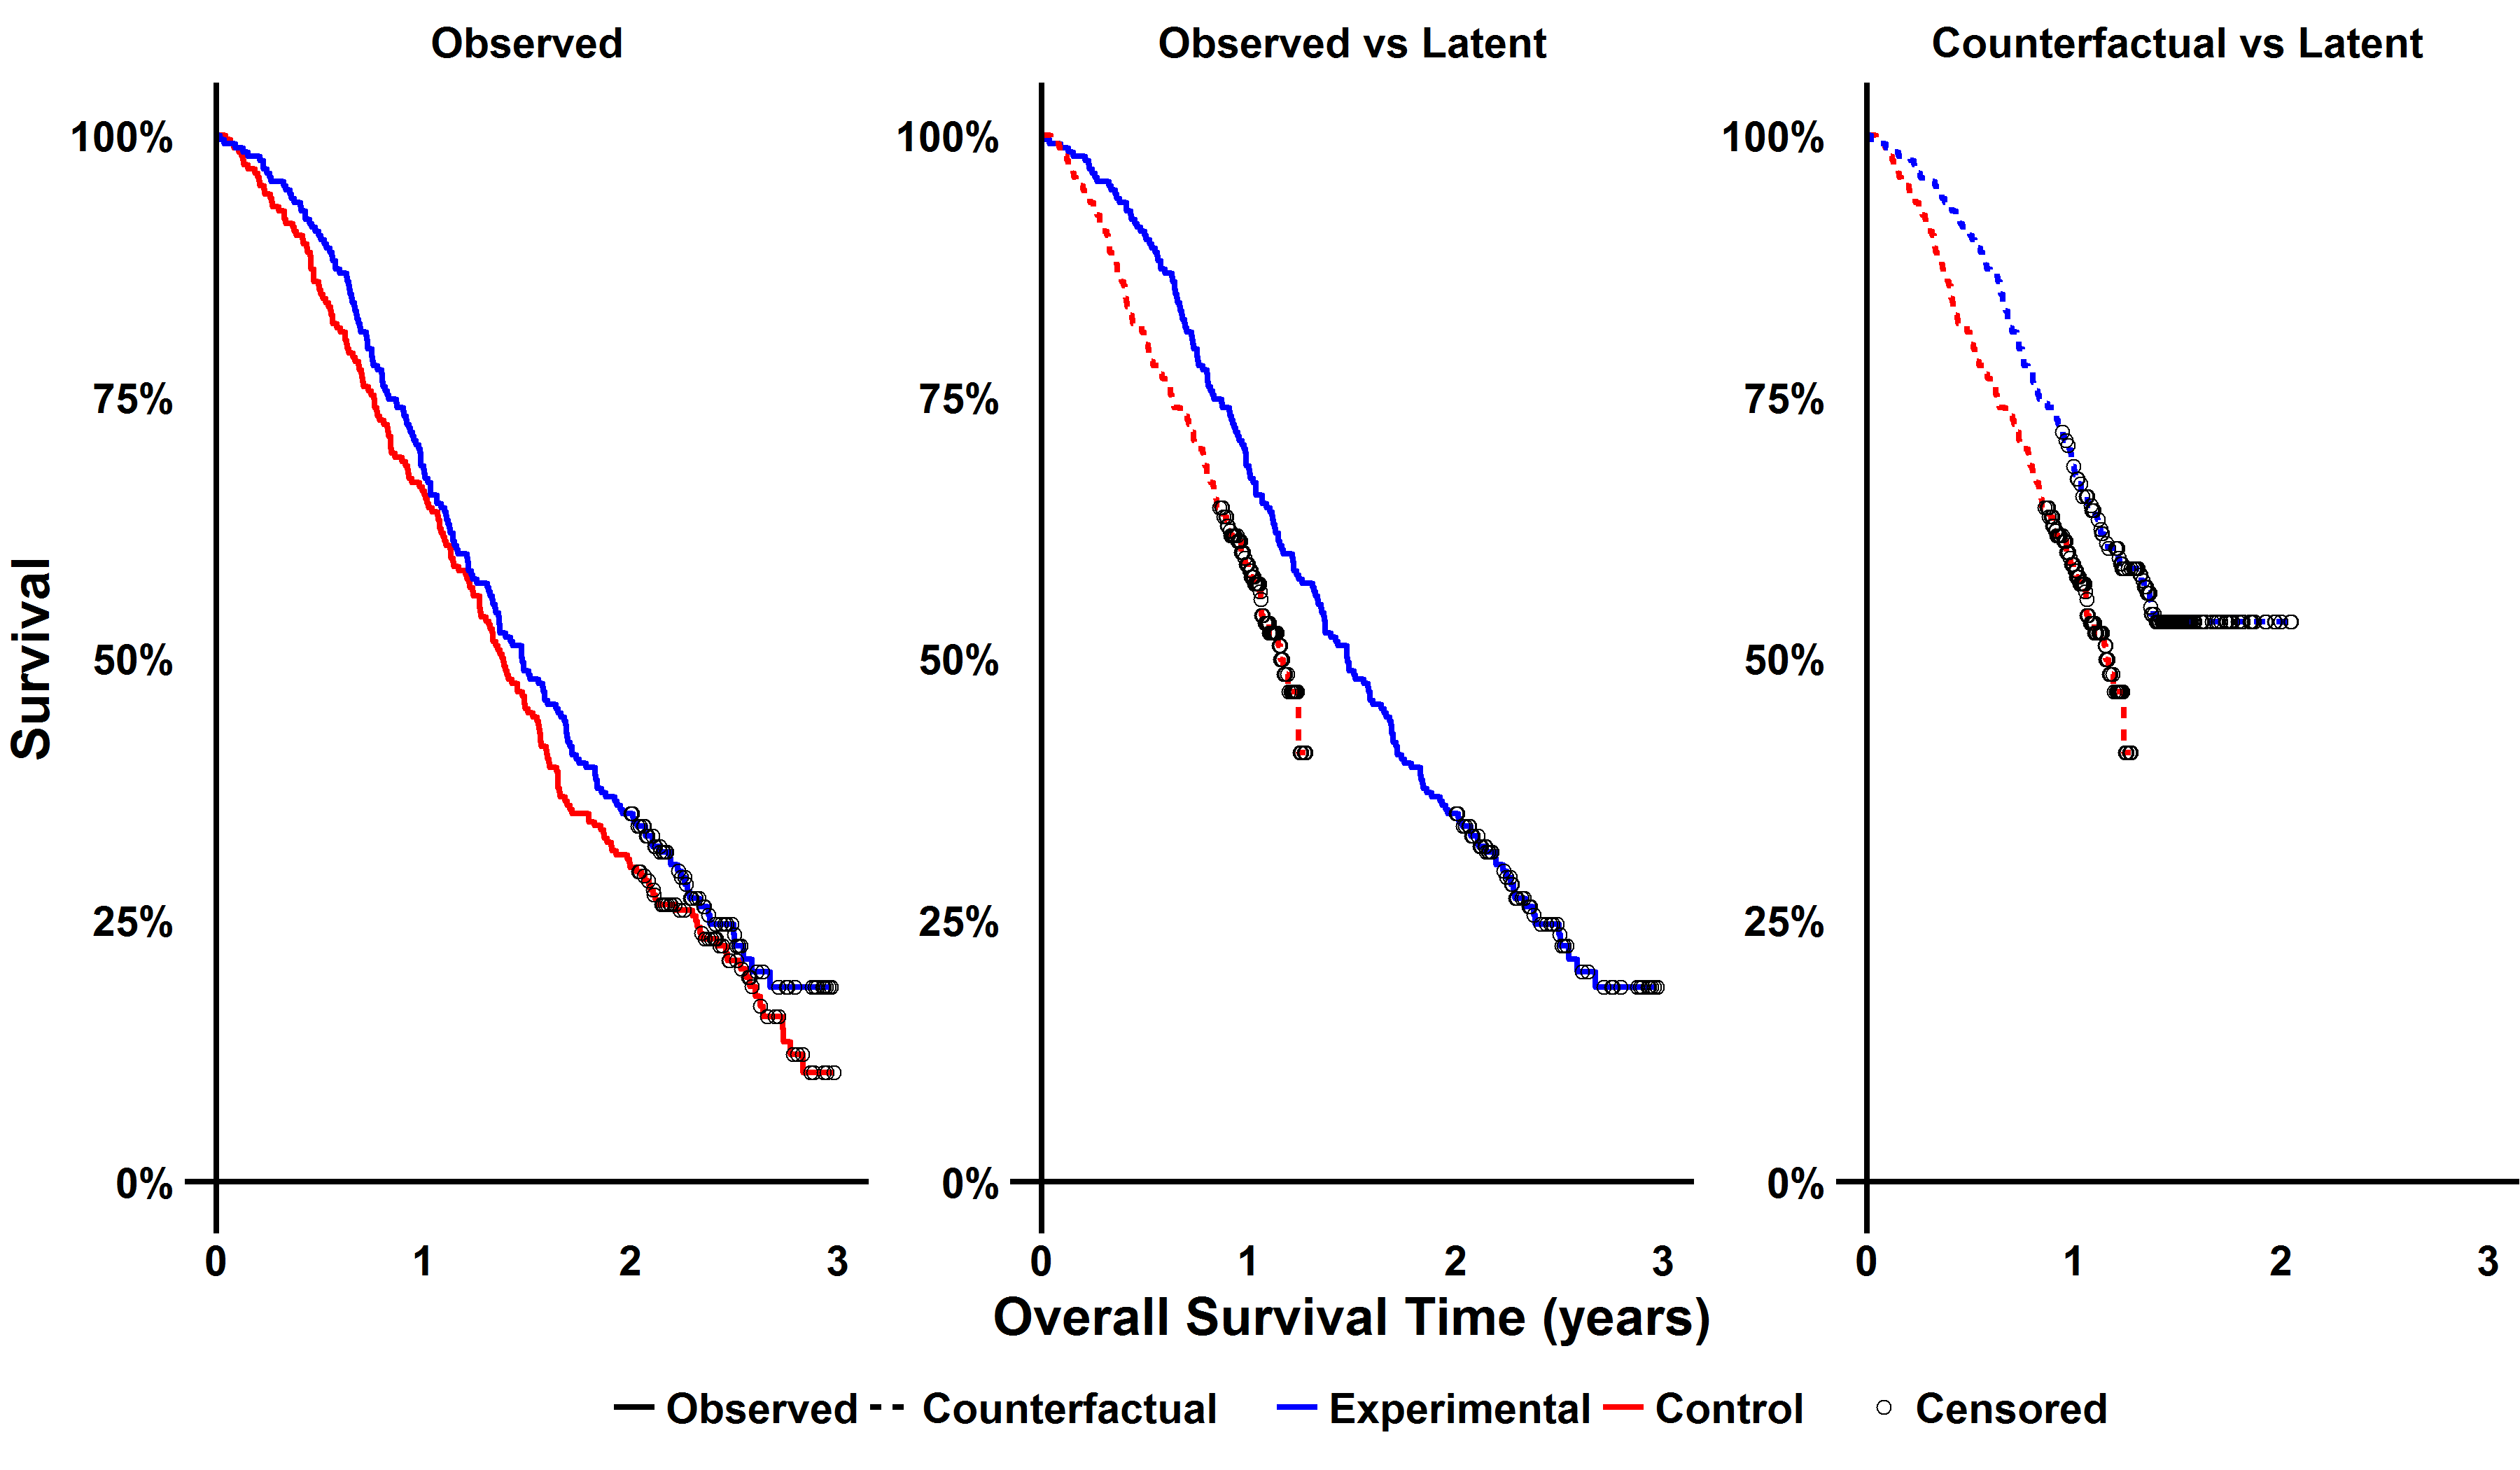
\includegraphics[width=15cm]{images/chap_methrev/example_cfact.png}
\caption{\label{F:methrev:excfact} Illustration of the different comparisons that can be made to derive corrected survival times for a simulated data set. the left panel shows the observed data $T_i$. The middle panel illustrates the comparison of $T_i$ and $U_i$ suggested by \cite{Latimer2014}. The right panel shows the comparison of $V_i$ suggested by \cite{Robins1991} where for the experimental arm the observed treatment history is applied to the latent survival time.} 
\end{figure}





Regardless of approach taken once counter-factual survival times have been estimated they can be used to estimate other counter-factual statistics such as a Hazard Ratio by fitting a Cox model. \cite{White1999} notes that while point-estimates can be taken directly from the model ``The $p$-values and standard errors from this model do not reflect the uncertainty in the accelerated life model parameter''. Indeed they suggest to either bootstrap confidence intervals or construct ``symmetrical confidence intervals for the log hazard ratio using the ITT $p$-values''. This can be done by deriving the standard error as $SE(\hat{\beta}) = \frac{\hat{\beta}}{Z(0)}$ where $\hat{\beta}$ is the log hazard ratio estimated from the counter-factual Cox model and $Z(0)=Z(\psi|\psi=0)$ is the standard normal value from the rank test used in the g-estimation process for the ITT comparison.




\section{Iterative Parameter Estimation (IPE)}


\cite{Branson2002} propose another randomization based approach which uses a similar modelling framework to the RPSFT model by relating observed survival time ($T_i$) with an unobserved latent survival time ($U_i$). This relationship is defined by the model in Equation \ref{E:BWIPE} where $A_i$ is the time a patient starts experimental therapy.
\begin{equation}
U_{i} = A_i + e^{-\eta}( T_{i} - A_i )
\label{E:BWIPE}
\end{equation}
It can be seen that this is similar to the ``treatment group'' approach to RPSFT and makes the same common treatment effect assumption. 

\subsection{Parameter estimation}
The main difference with RPSFT is the approach taken to estimate the parameter $e^{-\eta}$. To do this it is assumed that the survival times follow a parametric accelerated failure time distribution such as a weibull. The parameter is then estimated in an iterative fashion as follows:
\begin{enumerate}
\item $\exp(-\hat{\eta}_1)$ is estimated by comparing the treatment arms as randomized using a parametric AFT model.
\item $U_{i,1}$ is estimated by using the estimate $\exp(-\hat{\eta}_1)$  in Equation  \ref{E:BWIPE}. \label{step1}
\item $\exp(-\hat{\eta}_j)$  is estimated by comparing the $T_i$ for patients randomized to experimental treatment with the $U_{i,j-1}$ for patients randomized to control therapy using a parametric AFT model. 
\item The estimates $\exp(-\hat{\eta}_j)$ and $\exp(-\hat{\eta}_{j-1})$  are compared and if close enough\footnote{\cite{Branson2002} suggest a tolerance of $10^{-5}$.} the algorithm is said to have converged. If the algorithm does not converge then $U_{i,j}$ is estimated by substituting $\exp(-\hat{\eta}_j)$ into Equation \ref{E:BWIPE}. Steps 3 to 4 are then repeated until convergence is reached.
\end{enumerate}

\subsection{Handling Censored Data}
\label{S:chap_methrev:MIPE}

\cite{Branson2002} claim, that unlike RPSFT, ``IPE requires recensoring survival times only if they are projected beyond the end of the study. Consequently, the occurrence of recensoring is limited to those patients who switch treatment in the control arm, and will be required only if experimental treatment is detrimental compared with control.''

\cite{White2006} and \cite{Zhang2016} challenge this approach and argue that the same censoring rules on the latent survival ($U_i$) time scale need to be implemented as used for RPSFT. That is the estimated latent survival times for all control arm patients $U_{i,j-1}$ need to be recensored not just those of switchers. The recensoring time for a patient is dereived identically to RPSFT as $C_i^\star$ calculated with Equation \ref{E:MIPEcens} where $C_i$ is the patients known potential administrative censoring time. This implementation of IPE with corrected censoring rules is referred to by \cite{Zhang2016} as the modified IPE (MIPE).

\begin{equation}
\label{E:MIPEcens}
C_i^\star(\eta) = \min \left( C_i, C_i e^{-\eta} \right)
\end{equation}

\subsection{Estimating a corrected Hazard Ratio}

Estimation of a corrected Hazard Ratio follows the same procedure as with the RPSFT method with the choice being to take these from the parametric model directly\footnote{Assuming a Weibull is used which has both an proportional hazards and accelerated failure time interpretation.} or by doing a comparison of the $T_i$ for the experimental arm with the $U_i$ for the experimental arm. Similarly to RPSFT it is noted by \cite{Zhang2016} that care has to be taken with estimating confidence intervals.
\begin{quote}
Although it is relatively easy to calculate the point estimate [of treatment effect], the calculation of its variance (and CI) is not straightforward. It is not valid to use the variance and CI from the last iteration from the MIPE algorithm because it does not incorporate the variability of the point estimate from the previous iteration. Instead, the bootstrap method is usually recommended.
\end{quote}

\section{Two Stage Accelerated Failure Time (AFT) model }

\cite{Latimer2013} introduce a simplified observational method that requires less data than the IPCW. The approach is too assume there is a single timepoint when all patients have a choice to switch or not switch and to define a secondary baseline at this timepoint. For all control arm patients who reach this ``second baseline'' they are designated as switcher/nonswitcher and compared, adjusting for other covariates measured at the ``second baseline'' in an AFT model to get an adjusted estimate for the effect of switch treatment. As an AFT model is used, the survival time for the patients who switch can be shrunk using this estimate of treatment effect. In practice given the design of oncology trials this this method is usually applied with time of progression  taken as the ``second baseline'' though as noted in Section \ref{S:chap_intro:pattern} this pattern of switching may not always apply. 

\subsection{Estimating counterfactual survival}

Estimation of the counterfactual survival time is done by partitioning the overall survival time for control arm patients into progression free survival (PFS) and survival post progression (SPP) as shown in Figure \ref{F:chap_intro:pfsandpps}. A parametric AFT model is then fit to the SPP times adjusting for covariates captured at the time of progression as shown in Equation \ref{E:chap_meth:2saftm1} where $X_{SWITCH}$ is the indicator for switch and $X_1 \ldots X_p$ are the additional covariates to adjust for.

\begin{align}
S(t_{SPP}; \theta) &= S_0(\theta t_{SPP}) \label{E:chap_meth:2saftm1} \\
\theta &= \exp(-[\eta X_{SWITCH} + \beta_1 X_1 + \ldots + \beta_p X_p]) \nonumber
\end{align}

The counterfactual survival time ($U_i$) for a patient $i$ can then be defined as shown in Equation \ref{E:chap_meth:2saftm2} similarly to the RPSFT and IPE methods.
\begin{equation}
U_i = T_{PFS_i} + T_{SPP_i} e^{-\eta}  \label{E:chap_meth:2saftm2}
\end{equation}

It is important to note that this approach will only yield correct estimates if the model shown in Equation \ref{E:chap_meth:2saftm1} is correct and all covariates that could influence survival are collected at the time of progression.

\subsection{Handling Censored Data}
\label{S:chap_meth:2saftcens}
\cite{Latimer2016} note that as this method is defining a counterfactual survival time the same concerns around informative censoring on  the counterfactual time scale as discussed for the RPFST and MIPE methods apply. As such they advocate censoring the $U_i$ at $C_i^\star(\eta)$ defined as shown in Equation \ref{E:chap_meth:2saftcens} where as before $C_i$ is the patients known potential administrative censoring time.
\begin{equation}
\label{E:chap_meth:2saftcens}
C_i^\star(\eta) = \min \left( C_i, C_i e^{-\eta} \right)
\end{equation}
It can be seen that this is perhaps a conservative approach as it makes the assumption that each control arm patient could potentially be on switch treatment for the whole of their follow-up period which is clearly not possible. A potential alternative censoring mechanism which would require less observations to be censored is as shown in Equation \ref{E:chap_meth:2saftcens2} where $K$ is the potential minimum switching time (such as the shortest PFS time observed within the trial).
\begin{equation}
\label{E:chap_meth:2saftcens2}
C_i^\star(\eta) = \min \left( C_i, K + (C_i - K) e^{-\eta} \right)
\end{equation}

\subsection{Estimating a corrected Hazard Ratio}

Estimation of a corrected Hazard Ratio follows the same procedure as with the RPSFT and MIPE method by doing a comparison of the $T_i$ for the experimental arm with the $U_i$ for the control arm. As with the RPSFT and MIPE methods \cite{Latimer2016} note that confidence intervals need to be estimated through bootstrapping. 

\section{Summary}

In this Chapter a selection of methods that have been proposed to analyse trials where treatment switching has occurred are described. As discussed in Section \ref{S:chap_intro:simstudy} an approach to assess the performance of these methods is to test each method against simulated data where a known treatment effect exists. This will be the focus of the reminder of this dissertation. 


